\addcontentsline{toc}{chapter}{Introduzione}
\chapter*{Introduzione}
	\markboth{Introduzione}{}
	Il mondo moderno è ormai pervaso dalla \emph{crittografia}. Quotidianamente e spesso inconsapevolmente utilizziamo funzioni crittografiche per le normali operazioni della vita quotidiana. Controllare il conto sull'home-banking, scambiarsi messaggi tramite servizi di messaggistica o anche navigare in internet utilizzando il protocollo \acs{HTTPS} sono azioni che svolgiamo ormai con naturalezza. I sistemi moderni rendono trasparente all'utente l'utilizzo di tali tecnologie, ma ciò non vuol dire che esse non esistano.
	
	Una \emph{funzione crittografica}\index{Funzione crittografica} è un oggetto matematico astratto che, attraverso l'utilizzo di una chiave, trasforma un dato in input (plaintext) in una sua rappresentazione diversa (ciphertext) il più possibile non riconducibile al dato originale. Questa funzione deve poi essere implementata in un programma che girerà su un \emph{dispositivo crittografico} in un certo ambiente, presentando perciò caratteristiche fisiche peculiari. Esempi di \dispp potrebbero essere smartcard, chiavette \acs{USB}, chip dedicati montati su dispositivi general purpose (smartphone, notebook) o periferiche progettate e costruite apposta per effettuare questo unico compito.
	
	In passato si guardava ad un \disps semplicemente come una black-box che riceveva un plaintext e restituiva un ciphertext (encryption) e viceversa (decryption) come in \cref{fig:blackbox}. Gli attacchi erano basati sulla conoscenza del ciphertext (ciphertext-only attacks) o di alcune coppie di entrambi (known plaintext attacks). Con l'accesso al meccanismo di encryption o di decryption, anche solo temporaneo, si possono attuare anche altri due tipi di attacchi (rispettivamente chosen-plaintext e chosen-ciphertext)\cite{dispenseCS}.
	
	\begin{figure}
		\begin{center}
			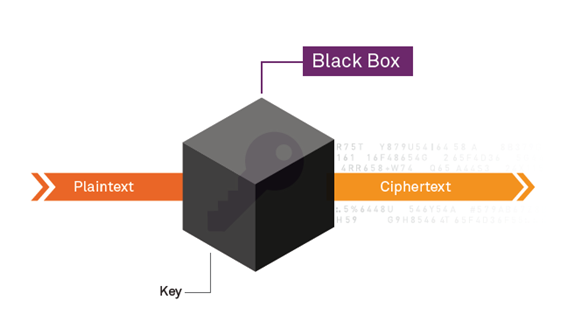
\includegraphics[width=\textwidth]{blackbox}
			\caption{black-box encryption}
			\label{fig:blackbox}
		\end{center}
	\end{figure}
	
	Al giorno d'oggi si è consapevoli del fatto che un \disps ha spesso altri input oltre al plaintext e altri output oltre al ciphertext. Gli input differenti dal plaintext possono essere le interazioni col mondo esterno come modifiche al voltaggio della corrente, condizioni atmosferiche particolari o sollecitazioni fisiche. Il nostro interesse sarà però focalizzato sulle informazioni (facilmente misurabili) che vengono lasciate trapelare dai dispositivi stessi oltre al ciphertext come ad esempio il tempo di esecuzione di un programma, le radiazioni emesse, suoni, luci e quant'altro chiamate \emph{side-channel informations}\index{Side-channel informations}.
	 
	 Il resto della tesi è organizzata nel seguente modo:
	 \begin{itemize}
	 	\item nel capitolo $1$, data l'eterogeneità della letteratura su questo argomento, abbiamo definito una classificazione dei side-channel attacks e abbiamo presentato una panoramica dello stato dell'arte.
	 	\item nel capitolo $2$ abbiamo focalizzato la nostra attenzione sulla categoria dei \emph{timing attacks}, una particolare tipologia di side-channel attack basato sull'osservazione del tempo di esecuzione di un programma. Partendo da alcuni timing attack reali eseguiti su particolari funzioni crittografiche, abbiamo ottenuto una generalizzazione applicabile a qualunque attacco di questo tipo.
	 	\item nel capitolo $3$ presentiamo i cache attacks, attacchi side-channel (prevalentemente di tipo timing) che colpiscono la memoria cache dei processori.
	 	\item nel capitolo $4$ abbiamo presentato approfonditamente il progetto \emph{SPECTRE}, la principale famiglia di timing attacks sulle cache, che affligge tutti i recenti processori AMD, ARM e Intel.
	 	\item nel capitolo $5$ descriviamo infine \ac{SPARK}, l'attacco da noi creato. Questo attacco, basato sui concetti del progetto SPECTRE, è in grado di ottenere dati protetti da password senza la conoscenza di quest'ultima.
	 \end{itemize}    
